\documentclass[notitlepage]{article}
\usepackage[utf8]{inputenc} 
\usepackage{geometry} 		
\usepackage{chngcntr}
\usepackage{amsmath} 			
\usepackage{amssymb}			
\usepackage{mathtools}		
\usepackage{comment} 			
\usepackage{mdframed}			
\usepackage{xcolor}				
\usepackage{fancyhdr}			
\usepackage{listings}			
\usepackage{color}				
\usepackage{tikz}	
\usepackage{tasks}			
\usepackage{exsheets}		
\usepackage{array}			
\usepackage{empheq}
\usepackage{caption}
\usepackage{pdfpages}
\usepackage{tabularx}

\geometry{ 						%Format titlepage (interrupted by newgeometry)
	a4paper,
	total={170mm,257mm}%,
	%left=0mm,
	%top=0mm,
}

%START DEFINE YOUR VARIABLES HERE

\newcommand{\documentName}{Project Initiation}
\newcommand{\projectName}{Label Refinement by Behavioral Similarity}

%END DEFINE YOUR VARIABLES HERE

\title{%
	\documentName\text{ } \\
  \large \projectName\text{ } \\
  }

\author{
	\large Document owner:\\
	Bianka Bakullari\\
	\texttt{}
	Christopher Beine\\
	\texttt{}
	Nicole Ventsch\\
	\texttt{}
	Juan\\
	\texttt{}
}

\date{\small{Last edited: \today}}

\pagestyle{fancy}
\fancyhf{}
\rhead{}
\lhead{\documentName\space-\space\projectName}

\makeatletter					%Prefix to add ToC to titlepage
\newcommand*{\toccontents}{\@starttoc{toc}}
\renewcommand*\contentsname{}
\makeatother
                  

\begin{document}

\begin{titlepage}
\clearpage\maketitle			%Clear title page
\thispagestyle{fancy}
\tableofcontents
\end{titlepage}

\rfoot{\thepage}				%Start printing page-numbers, after title page.

\newgeometry{ 					%Default page formatting on-going #1
	total={170mm,257mm},
	left=20mm,
	top=25mm,
    bottom=30mm					%Causes warning
}

\begin{flushleft}				%Default page formatting on-going #2

\section{Overview}
Many processes involve carrying out an action multiple times. An example for this would be an online shop in which you first have to pay a registration fee before ordering an item and paying it. This process contains the event "payment" twice, but in different contexts, so that the payments are actually two different tasks. In the context of analysing processes, the event logs usually only contain the event names, so that the "payment" actions would be treated as the same task and loops would be induced in the resulting models. However, these loops do not match the actual process, which is the issue this project addresses. 

These imprecise logs should be refined based on the structural contexts of the events. We want to refine the logs without any filtering. Moreover, we want to allow an interactive change of the thresholds used to refine the labels since this can differ for every log and we have no knowledge of the correctness of the refined log in general.

By designing an interface that allows the users to upload an event log, to set the thresholds and to download the modified event log, carrying out this project will save the data analysts a lot of time which is needed to refine the log and will make their results more accurate.  Using this approach, the process logs can be refined to reach a higher precision in the subsequent analysis of up to $89 \, \% $, which highly increases the quality of the process discovery results. These better results can lead to more optimized processes and that way reduce the company's expenses while increasing its efficiency. 


\section{Business Case}

\subsection{Intial situation}

\subsection{Scope}

During the project, we will create both code and documentations. Thus, the scope will be divided into these two aspects:

Documentation: 
\begin{itemize}
	\item develop and describe the design of the interface we will use and picture how users can set the thresholds in the interface 
	\item design the algorithm structure by stating the usage of classes as well as the inputs and outputs for the functions that are used
	
\end{itemize} 


Implementation:
\begin{itemize}
	\item set up a Web Service based on Python that uses the label refinement algorithm proposed by Xixi Lu, et al.
	\item create a user interface that allows the users to upload the original event log, set thresholds and imprecise label scope and finally download the refined event log
\end{itemize}

\subsection{Key Benefits}

\subsection{Assumptions}

In this project we will assume that an event log is given by the user, i.e., data that contains at least the attributes "id", "time stamp" and "activity name". Moreover, we will assume that these event logs are given in the standard XES format. 

\section{Feasibility study}

\subsection{Theoretical point of view}

From a theoretical point of view, we view an event log for which we suspect to have different tasks being handled as the same activity as \textit{imprecise}.
In reality, each event in the data is a unique occurrence over time.
By defining a \textit{labeling  function} which maps these events to a finite set of activity names, also called \textit{labels}, we obtain event logs having common activities across traces and within traces.
A problem arises when similar events happening in different contexts are assigned the same label.
Applying process discovery algorithms to such event logs may lead to process models being imprecise, misleading or even incorrect.

There has already been some research investigating this problem. 
Some of the approaches include using additional domain knowledge to correct the labeling, or trace clustering to do relabeling according to the different variants.

In our project, we focus on the algorithm developed, investigated and explained in [paper], which given an event log, refines the labels of events based only on the context and patterns present in this event log.
The approach consists of three main steps: 1)detecting activities which need refined labels, do relabeling 2)accross dissimilar traces and then 3)within traces.
In our project, we assume that the set of activities needing relabeling is given and the user should have the possibility to set the thresholds affecting the relabeling in steps 2) and 3).

Since the logs have a finite set of activities leaving room for only a reduced number of computations needed for the cost function in step 2) and the fact that this algorithm has already been successfully implemented in ProM yielding good results, we conclude that the project is feasible from a theoretical point of view.\\

\subsection{Technical point of view}

As stated in [paper], the algorithm has already been implemented in ProM, where controlled experiments have been made to test the performance of the algorithm based on event logs containing different patterns.
There has also been a real life case study involving an event log with data concerning healthcare which was provided by Maastricht University Medical Center (MUMC+), a large academic hospital in the Netherlands.
In the log containing 1039 cases and 6213 events, the activities \textit{surgery} and \textit{consultation} were imprecise.
After relabeling, the resulting model reflected the behaviour which was described by the domain experts, according to whom the acitivity \textit{surgery} for example took place many times during the treatment of certain patients.

For our project we will use Python as back-end programming language to implement the algorithm. 

\textcolor{red}{@all front end, libraries used and why}\\

{\color{gray} *************** under construction *****************}

{\color{red} @all Do we need external libraries to implement the algorithm?}\\
{\color{red} TODO: formulate bullet points [to be done until friday]}

\begin{itemize}
	\item Flask 1.0.2 as web application framework
	\item Python 3.7.2 as back-end programming language
	\item JavaScript as Front-end development language (Standard ECMAScript 2018)
	\item Browser support (Google Chrome version $\geq$ 70, Firefox version $\geq$ 63, Maybe don't support IE/Edge)
	\item {\color{red} TODO: Select HTML5 visualisation framework for petri nets [To be done until saturday]}
	\item {\color{red} TODO: Select JavaScript Framework / Actually Required? [To be done until saturday]}
	\item Bootstrap version 4.3.1 for fast ui design
\end{itemize}

\large{flask}
\begin{itemize}
	\item References: Netflix Lemur, Linked-in internal stack
	\item Minimalistic Framework
	\item highly customizable
\end{itemize}

\large{Python}
\begin{itemize}
	\item Specified by stackholder
	\item highly used for datascience
	\item reference
\end{itemize}

\large{JavaScript}
\begin{itemize}
	\item defacto standard
	\item Required for dynamic content
\end{itemize}

\large{Bootstrap}
\begin{itemize}
	\item References: Twitter, Spotify, Coursera
	\item Fast Responsive UI design (May indicate responsive as optional for project)
\end{itemize}

{\color{gray} **************************************************}


\subsection{Risks and migiations}

\subsubsection{Project management risks}

\begin{tabularx}{12cm}{|X|X|}
\hline
\textbf{Risks} &\textbf{Mitigations}\\
\hline
Misunderstanding of Tasks & Do regular discussiond, meetings in the group and with the project supervisor\\
\hline
Unmatching schedules of the team members & Arrange meetings in advance, notify other members for any change  \\
\hline
Acquiring new skills under time pressure & Assign tasks based on individual strengths to increase efficiency \\ 
\hline
\end{tabularx}\\ 


\subsubsection{Technical risks}

\begin{tabularx}{12cm}{|X|X|}
\hline
\textbf{Risks} &\textbf{Mitigations}\\
\hline
Inconsistencies in programming styles & Explain the code to other members, write useful comments while coding\\
\hline
Unclear performance measures & Test code on small event logs, use automatically generated event logs to experiment \\
\hline
Software components do not work as a whole & Put emphasis on the design step \\ 
\hline
\end{tabularx}






\section{Project Plan}

\subsection{Milestones}

The project starts on the 09/04/2019 and ends on the 08/07/2019 and is divided into nine milestones. The project is managed with a scrum-oriented approach
where each milestone represents a sprint. The project team organizes the required tasks during each sprint and visualize the current project status via a dashboard.

{\color{red} TODO: add sprint description until friday} \\
\begin{center}
	\captionof{table}{Overview Milestones }
  \begin{tabular}{ m{0.4cm} m{5cm} m{8.5cm} m{2cm} }
  	\hline
		ID & Milestone & Description & Deadline \\ \hline
		1 & Project Initiation document & The Project Initiation Document provides all of the key information required to start and run the project. This includes the project description, business case, feasibility study and a project team presentation.  & 19/04/2019 \\ \hline
		2 & Requirements Specification document & The Requirements Specification document contains functional and none functional requirements such as a set of use cases to describe the system interactions. & 29/04/2019 \\ \hline
		3 & Design Analysis and dummy P.o.C. & The final document is a description about the planned system architectural background and a proof of concept visualizing the main UI components. & 13/05/2019 \\ \hline
		4 & Sprint 1 code and documentation & {\color{red} TODO: sprint description depending on GANTT chart}  & 24/05/2019 \\ \hline
		5 & Sprint 2 code and documentation & {\color{red} TODO: sprint description depending on GANTT chart} & 07/06/2019 \\ \hline
		6 & Sprint 3 code and documentation & {\color{red} TODO: sprint description depending on GANTT chart} & 21/06/2019 \\ \hline
		7 & Testing, assessment and deployment & The application is checked for accuracy and should be aviable for use. & 01/07/2019 \\ \hline
		8 & Final report on the project & The final report provides an overview about the project course and the result. & 08/07/2019 \\ \hline
	\end{tabular}
\end{center}

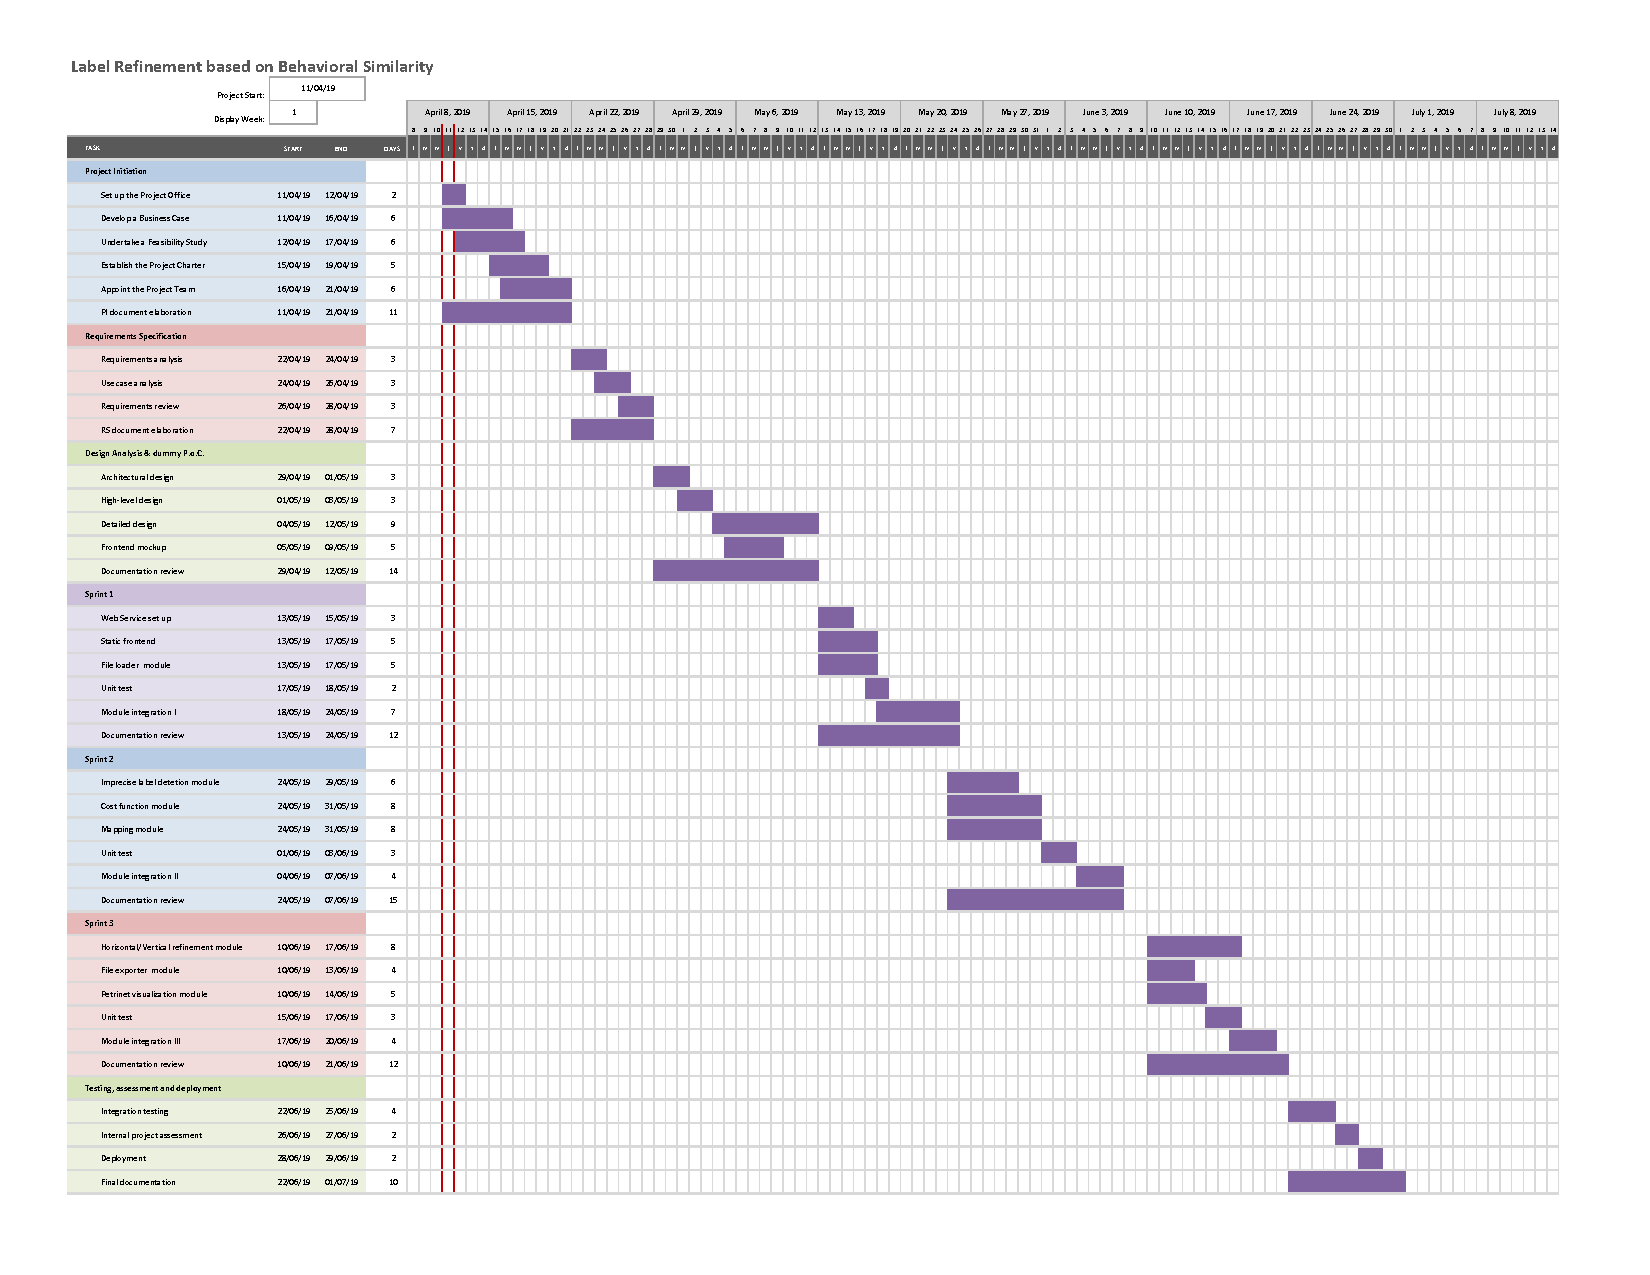
\includepdf[landscape=true]{ganttChart.pdf} 

\subsection{Deliverables}
With each milestones various deliverables are created to monitor, document and verify the docuemnt progress.
\newline
\textbf{1 Project Initiation document:}
\\
\begin{itemize}
	\item Finale project initiation document with key information about the project
\end{itemize}

\textbf{2 Requirements Specification document:}
\\
\begin{itemize}
	\item Requiredments Specification document with functional und none functional requirements
	\item Use case analysis
\end{itemize}

\textbf{3 Design analysis and dummy P.o.C:}
\\
\begin{itemize}
	\item System and software architecture documentation
	\item Frontend mockup
\end{itemize}

\textbf{4 Sprint 1 code and documentation }
\\
\begin{itemize}
	\item Python components
	\item Unit Test protocols
	\item Code documentation
\end{itemize}

\textbf{5  Sprint 2 code and documentation }
\\
\begin{itemize}
	\item Python components
	\item Unit Test protocols
	\item Code documentation
\end{itemize}

\textbf{6 Sprint 3 code and documentation }
\\
\begin{itemize}
	\item Python components
	\item Java Script components
	\item Unit Test protocols
	\item Code documentation
\end{itemize}

{\color{red} @all: should we write tests during the implementation? Could possibly save us a lot of trouble, but we have to select a test framework.
Otherwise we can remove the Unit Test protocols}

\textbf{7 Testing, assessment and deployment}
\\
\begin{itemize}
	\item Testprotocols
	\item Server configuration
	\item Web API 
	\item Webapplication
\end{itemize}

\textbf{8 Final report on the project}
\\
\begin{itemize}
	\item Final report
\end{itemize}

{\color{red} @all: Any other documents, reports, protocols or code artefacts required?}

\subsection{Timetable}

\section{Project Team}

\subsection{Competences} 
% May include self assement here 
\subsubsection{Nicole Ventsch}

I am a Master student studying Mathematics and Data Science in parallel.  Moreover, I work as a student assistant in the field of Data Analytics / Business Intelligence. Due to my background in mathematics, I have a good understanding of theoretical foundations. Moreover, I am very interested in Data Science and already took many courses in that area. Since I took the course "Introduction to Data Science", I also worked with Python before, so that I should be able to implement an algorithm in Python.

Though I have a strong theoretical background, I never worked on user interfaces or with web services, so that this aspect of the project could be challenging for me. 

\subsection{Juan Garza}

Juan Garza is a student at the RWTH University. He is currently in his 4th semester of studies towards a master’s degree in computer science. During his studies, he deepened his knowledge of process mining by attending the lecture “Business Process intelligence”. Moreover, he carried out a seminar on “Selected Topics in Process Mining”. He is familiar with Java and Python as programming languages. Besides school projects, he has no programming experience in “real world” environments which may represent a difficulty for him. 

\subsection{Roles}

\section{Project office}

\subsection{Description}

\end{flushleft}

\end{document}